\documentclass{standalone}

\usepackage[euler-digits]{eulervm}

\usepackage{tikz}
\tikzset{every node/.style={regular polygon,regular polygon sides=5,align=center,draw,shade,minimum size=22mm,inner sep=0pt}}
\tikzset{every path/.style={->,>=latex}}
\tikzset{t/.style={rectangle}}
\tikzset{r/.style={top color=red}}
\tikzset{g/.style={top color=green}}
\tikzset{b/.style={top color=blue}}

\usetikzlibrary{shapes}

\begin{document}
    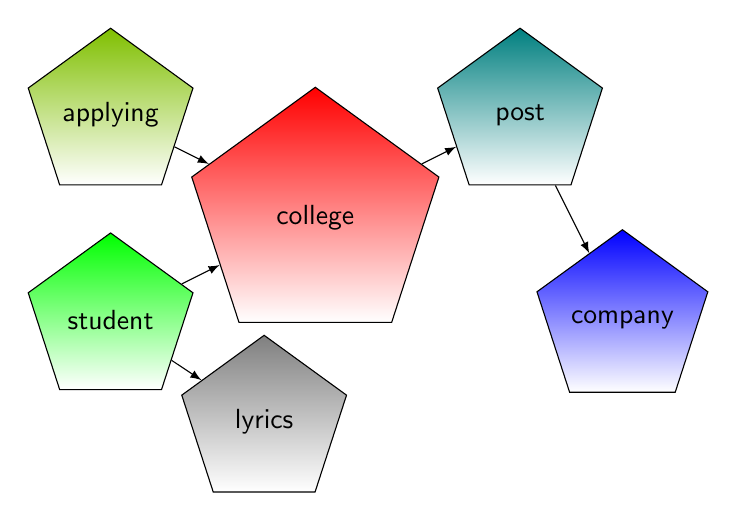
\begin{tikzpicture}[font=\sffamily,scale=1.3]
\node[r,minimum size=33mm](college) at (0,0) {college};
\node[top color=green!50!orange](apply) at (-2, 1) {applying};
\node[g](student) at (-2,-1) {student};
\node(lyrics) at (-0.5, -2) {lyrics};

\node[top color=blue!50!green](post2) at (2,1) { post};
\node[b](company) at (3,-1) {company};

\draw (student) -- (college);
\draw (student) -- (lyrics);
\draw (apply) -- (college);
\draw (college) -- (post2);
\draw (post2) -- (company);

    \end{tikzpicture}
\end{document}
